\section{Agent Backend Implementation}
\label{sec:agent-backend}

This section describes the implementation of the agent backend, which orchestrates the multi-agent system and manages communication between the frontend, LLM API, and MCP server. The design decisions presented here reflect careful consideration of safety, usability, and architectural clarity in the context of HPC cluster management.

\subsection{Technology Stack}

The backend is implemented using Python 3.10+ as the primary language, selected for its extensive ecosystem of AI and asynchronous programming libraries. The core technology stack includes:

\begin{itemize}
    \item \textbf{OpenAI Agents SDK} \cite{openaiagentssdk2024}: Foundational framework for agent implementation, offering built-in support for tool calling, conversation management, and multi-agent orchestration
    \item \textbf{FastAPI} (v0.116+) \cite{fastapi2024}: High-performance asynchronous web framework enabling efficient handling of concurrent requests
    \item \textbf{Uvicorn}: ASGI server for production deployment
    \item \textbf{Pydantic}: Structured output validation and command parameter modeling
    \item \textbf{SQLite}: Persistent storage for session management, conversation history, and pending actions
    \item \textbf{MCP Client Library}: Establishes the connection to the MCP server via SSE transport \cite{sse2024}
    \item \textbf{SSE-Starlette}: Provides streaming infrastructure for real-time response delivery to the frontend in OpenWebUI-compatible format
\end{itemize}

\subsection{Multi-Agent Architecture: Sub-Agents as Tools}

A critical architectural decision in this implementation is the use of specialized sub-agents implemented as callable tools rather than as simple function-based tools \cite{wu2023autogen}. This design choice addresses several challenges inherent in HPC cluster management operations.

\subsubsection{Rationale for Sub-Agent Design}

Traditional tool-based architectures assume that each tool performs a discrete, well-defined operation with predictable input-output patterns \cite{schick2023toolformer}. However, Slurm cluster operations frequently require complex reasoning chains that simple tools cannot adequately support. For example, analyzing job failures requires not only retrieving job data via \texttt{sacct}, but also correlating that data with node status from \texttt{sinfo}, examining recent configuration changes, and potentially searching documentation for error codes. This multi-step reasoning process exceeds the capabilities of a single function tool.

By implementing the Analysis Sub-Agent and Action Sub-Agent as dedicated agents rather than simple functions, the system gains several advantages. First, each sub-agent maintains its own instruction set optimized for its specific domain, enabling focused reasoning without the cognitive overhead of a monolithic prompt. Second, sub-agents can autonomously chain multiple MCP tool calls within a single invocation, performing iterative data gathering without returning to the main agent after each step. Third, tool isolation prevents the main agent from being overwhelmed by the full complexity of all available Slurm commands, instead presenting a simplified interface of ``analyze the cluster'' and ``manage jobs.''

\subsubsection{Tool Access Control}

A key architectural feature is strict tool isolation between agents. Table~\ref{tab:agent-tools} shows the complete tool access matrix.

\begin{table}[H]
    \centering
    \caption{Agent Tool Access Matrix}
    \label{tab:agent-tools}
    \small
    \begin{tabular}{|l|c|c|c|l|}
        \hline
        \textbf{Tool} & \textbf{Main} & \textbf{Analysis} & \textbf{Action} & \textbf{Confirmation} \\
        \hline
        \multicolumn{5}{|l|}{\textit{Query Tools}} \\
        \hline
        \texttt{squeue} & & \checkmark & \checkmark & No \\
        \texttt{sacct} & & \checkmark & \checkmark & No \\
        \texttt{sinfo} & & \checkmark & \checkmark & No \\
        \texttt{scontrol\_show} & & \checkmark & \checkmark & No \\
        \texttt{run\_analysis} & & \checkmark & & No \\
        \texttt{web\_search} & & \checkmark & & No \\
        \texttt{sacctmgr\_show} & & & \checkmark & No \\
        \texttt{sreport} & & & \checkmark & No \\
        \hline
        \multicolumn{5}{|l|}{\textit{Action Tools}} \\
        \hline
        \texttt{sbatch} & & & \checkmark & Yes \\
        \texttt{scancel} & & & \checkmark & Yes \\
        \texttt{scontrol\_hold} & & & \checkmark & Yes \\
        \texttt{scontrol\_release} & & & \checkmark & Yes \\
        \texttt{scontrol\_update} & & & \checkmark & Yes \\
        \texttt{scontrol\_requeue} & & & \checkmark & Yes \\
        \texttt{srun} & & & \checkmark & No \\
        \texttt{salloc} & & & \checkmark & No \\
        \hline
        \multicolumn{5}{|l|}{\textit{Admin Tools}} \\
        \hline
        \texttt{scontrol\_create/delete} & & & \checkmark & Yes \\
        \texttt{scontrol\_reconfigure} & & & \checkmark & Yes \\
        \texttt{sacctmgr\_add/modify/delete} & & & \checkmark & Yes \\
        \hline
        \multicolumn{5}{|l|}{\textit{Main Agent Direct Tools}} \\
        \hline
        \texttt{analyze\_cluster} (sub-agent) & \checkmark & & & No \\
        \texttt{manage\_jobs} (sub-agent) & \checkmark & & & No \\
        \texttt{generate\_chart} & \checkmark & & & No \\
        \texttt{confirm\_action} & \checkmark & & & No \\
        \texttt{cancel\_action} & \checkmark & & & No \\
        \hline
    \end{tabular}
\end{table}

\subsubsection{Analysis Sub-Agent Specification}

The Analysis Sub-Agent is designated for read-only data gathering operations. When the main agent determines that cluster investigation is needed, it invokes the Analysis Sub-Agent with a natural language request such as ``investigate why jobs in partition gpu are pending.'' The sub-agent autonomously determines which tools to call, chains multiple queries if needed, and returns a structured summary for synthesis into a user-facing response.

\subsubsection{Action Sub-Agent Specification}

The Action Sub-Agent handles operations that modify cluster state. The segregation of action-oriented operations into a dedicated sub-agent serves both safety and clarity purposes. The Action Sub-Agent's instructions emphasize verification requirements and consequence awareness, ensuring that potentially destructive operations receive appropriate scrutiny before execution. Dangerous operations are intercepted by the confirmation mechanism before reaching actual execution.

\subsubsection{Agent Prompt Engineering}

Each agent in the multi-agent system has carefully crafted instruction prompts that define its behavior, capabilities, and output format. These prompts are critical for ensuring reliable operation within the HPC cluster management context.

\paragraph{Main Agent Prompt Design}

The main agent serves as the orchestrator and user-facing interface. Its prompt is structured into several key sections:

\begin{itemize}
    \item \textbf{Critical Rules}: Establishes behavioral constraints, most importantly the rule to ``ALWAYS call tools first'' rather than fabricating information. This prevents hallucination of cluster status.
    \item \textbf{Tool Descriptions}: Documents available tools including \texttt{analyze\_cluster} for data gathering, \texttt{manage\_jobs} for actions, and \texttt{generate\_chart} for visualization.
    \item \textbf{Output Format Specification}: Defines structured table formats for presenting cluster status, job landscapes, and recommendations. This ensures consistent, scannable output.
    \item \textbf{Workflow Guidelines}: Provides step-by-step guidance for common scenarios such as web searches for debugging and cluster data analysis.
\end{itemize}

\paragraph{Analysis Sub-Agent Prompt Design}

The Analysis Sub-Agent uses a minimal, focused prompt optimized for tool execution rather than conversation:

\begin{itemize}
    \item \textbf{Single-Tool Invocation}: The prompt explicitly states ``Call ONE tool only, then stop,'' preventing unnecessary reasoning loops.
    \item \textbf{Semantic Tool Selection}: The prompt guides tool selection based on user intent rather than keyword patterns. Requests seeking external knowledge (troubleshooting, error explanations, documentation) route to the web search tool, while data-gathering requests route to analysis scripts.
    \item \textbf{Raw Output Policy}: Instructions to ``Return raw tool output - do not summarize'' ensures the main agent receives complete data for synthesis.
\end{itemize}

\paragraph{Action Sub-Agent Prompt Design}

The Action Sub-Agent prompt emphasizes operational precision:

\begin{itemize}
    \item \textbf{Tool Categorization}: Groups tools by function (job control, interactive, admin, accounting) for clarity.
    \item \textbf{Confirmation Awareness}: Explicit mention that ``Dangerous actions are queued for user confirmation'' ensures the sub-agent understands the two-factor flow.
    \item \textbf{Result Reporting}: Instruction to ``Return execution results'' maintains transparency for user feedback.
\end{itemize}

\paragraph{Model Selection Strategy}

The implementation uses different models for different agent roles:
\begin{itemize}
    \item \textbf{Reasoning Model}: Used by the main agent with higher temperature (0.7) for creative problem-solving and natural conversation.
    \item \textbf{Tool Model}: Used by sub-agents with low temperature (0.1) for deterministic, precise tool execution.
\end{itemize}

This separation ensures that user-facing responses benefit from natural language fluency while tool invocations remain reliable and predictable.

The complete query processing workflow, including the Think-Act-Observe loop, sub-agent invocation, and confirmation handling, is illustrated in Figure~\ref{fig:query-sequence}.

\begin{figure}[H]
    \centering
    \makebox[\textwidth][c]{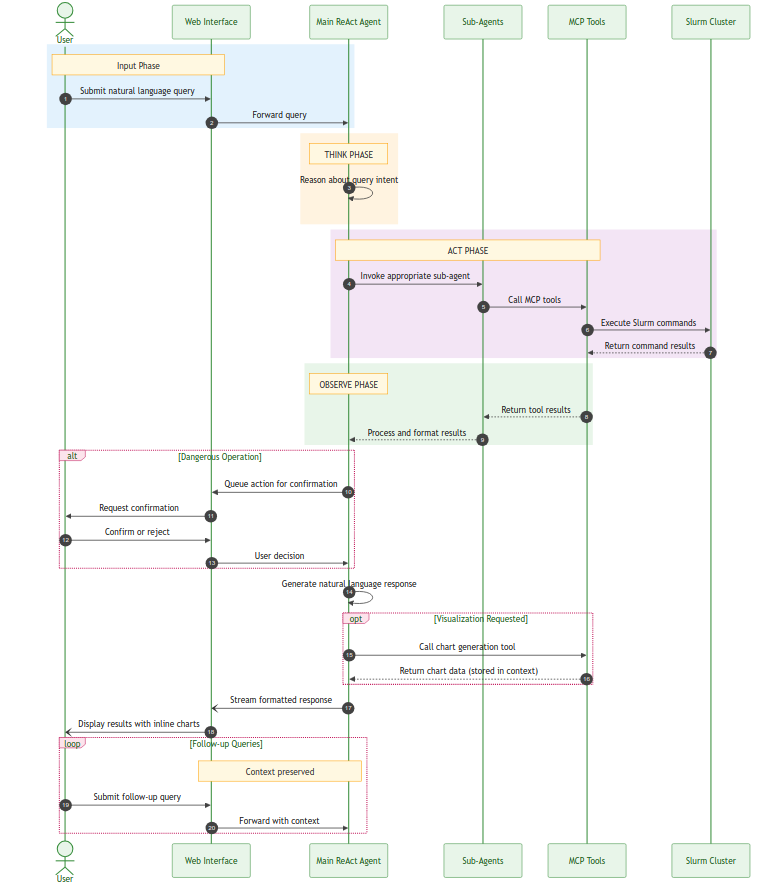
\includegraphics[width=1.3\textwidth]{images/react_agent_workflow.png}}
    \caption{Query Processing Sequence}
    \label{fig:query-sequence}
\end{figure}

\subsection{Confirmation Context: Two-Factor Authentication for Dangerous Operations}

The confirmation context mechanism prevents accidental execution of destructive operations. When a dangerous tool (e.g., \texttt{scancel}, \texttt{scontrol\_update}) is invoked, the system stores the pending action in SQLite rather than executing immediately, then returns a confirmation request to the user. This mirrors two-factor authentication: the first factor is the user's request, and the second is explicit confirmation.

Pending actions persist across session boundaries with automatic expiration after one hour. The confirmation tools (\texttt{confirm\_action} and \texttt{cancel\_action}) are available to the main agent, enabling natural conversational flow while enforcing the two-step verification process. The confirmation flow is illustrated in Figure~\ref{fig:confirmation-flow}.

\begin{figure}[H]
    \centering
    \makebox[\textwidth][c]{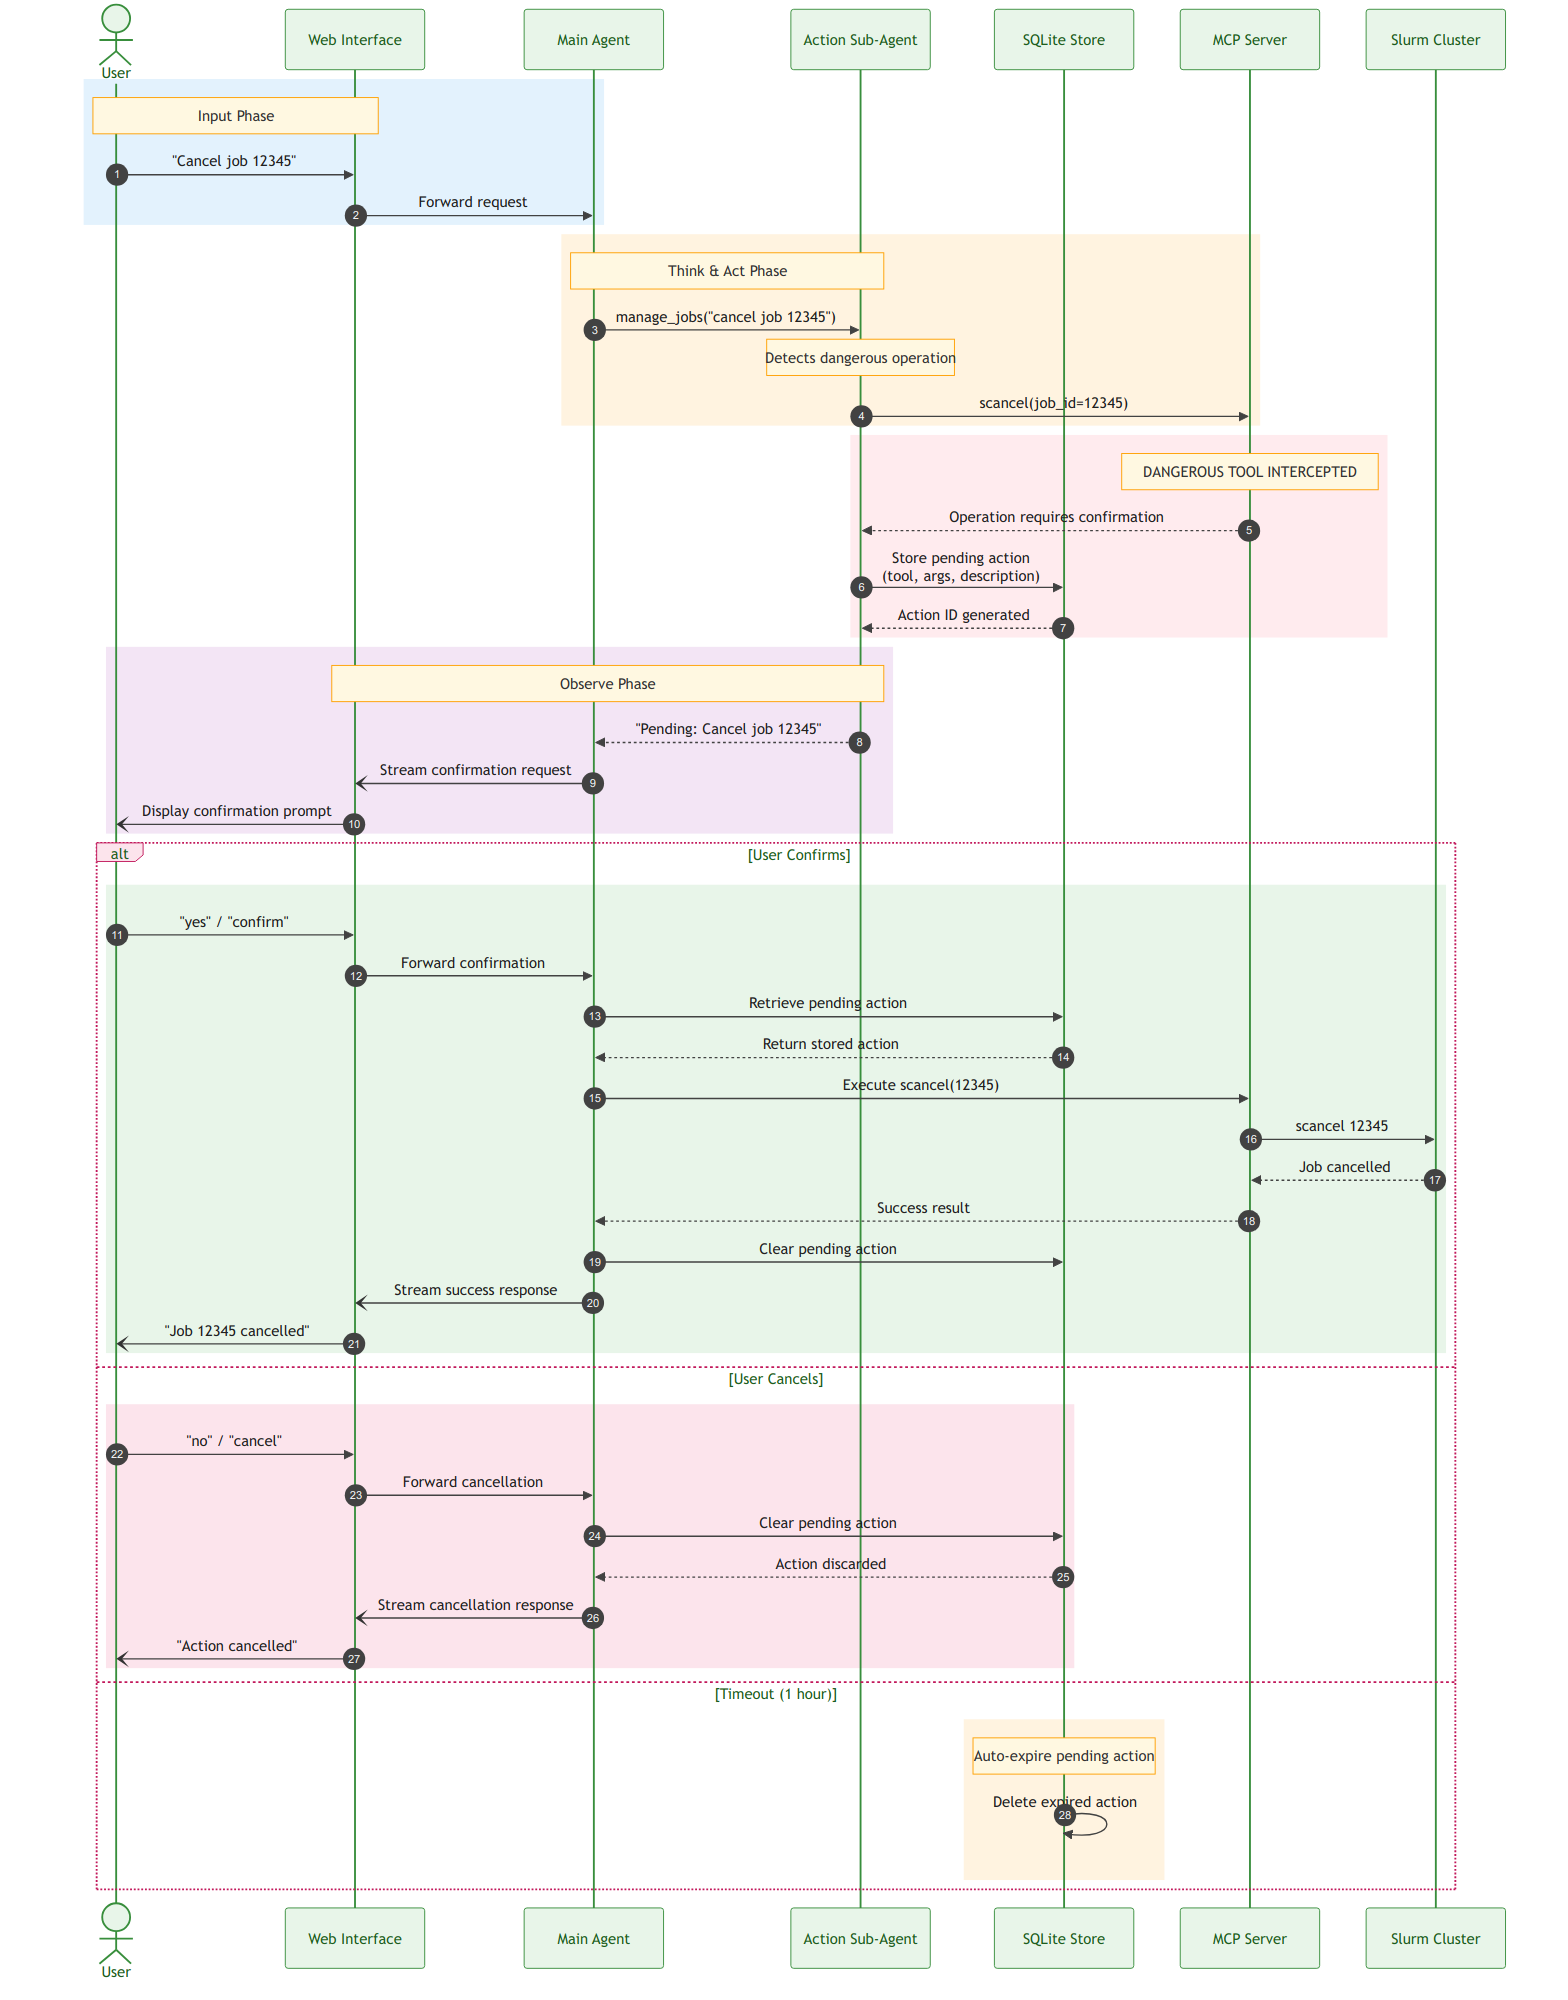
\includegraphics[width=1.3\textwidth]{images/confirmation_flow.png}}
    \caption{Two-Factor Confirmation Flow for Dangerous Operations}
    \label{fig:confirmation-flow}
\end{figure}

\subsection{Embedded Visual Handling: Chart Artifact Management}

Chart generation presents a unique challenge: base64-encoded images are thousands of characters long and would waste tokens if included in conversation history. The solution employs a multi-layer isolation strategy:

\begin{itemize}
    \item \textbf{Generation layer}: Chart tools return only a brief summary to the LLM while storing the actual image artifact in the run context
    \item \textbf{Streaming layer}: After LLM response completion, chart artifacts are appended with \texttt{[IMG]...[/IMG]} markers for frontend parsing
    \item \textbf{History layer}: A \texttt{ChartFilteredSession} wrapper strips chart artifacts from conversation history before subsequent LLM calls
\end{itemize}

Figure~\ref{fig:chart-artifact-flow} illustrates this isolation mechanism, showing how chart data flows through the system while keeping large artifacts separated from the conversation context.

\begin{figure}[H]
    \centering
    \makebox[\textwidth][c]{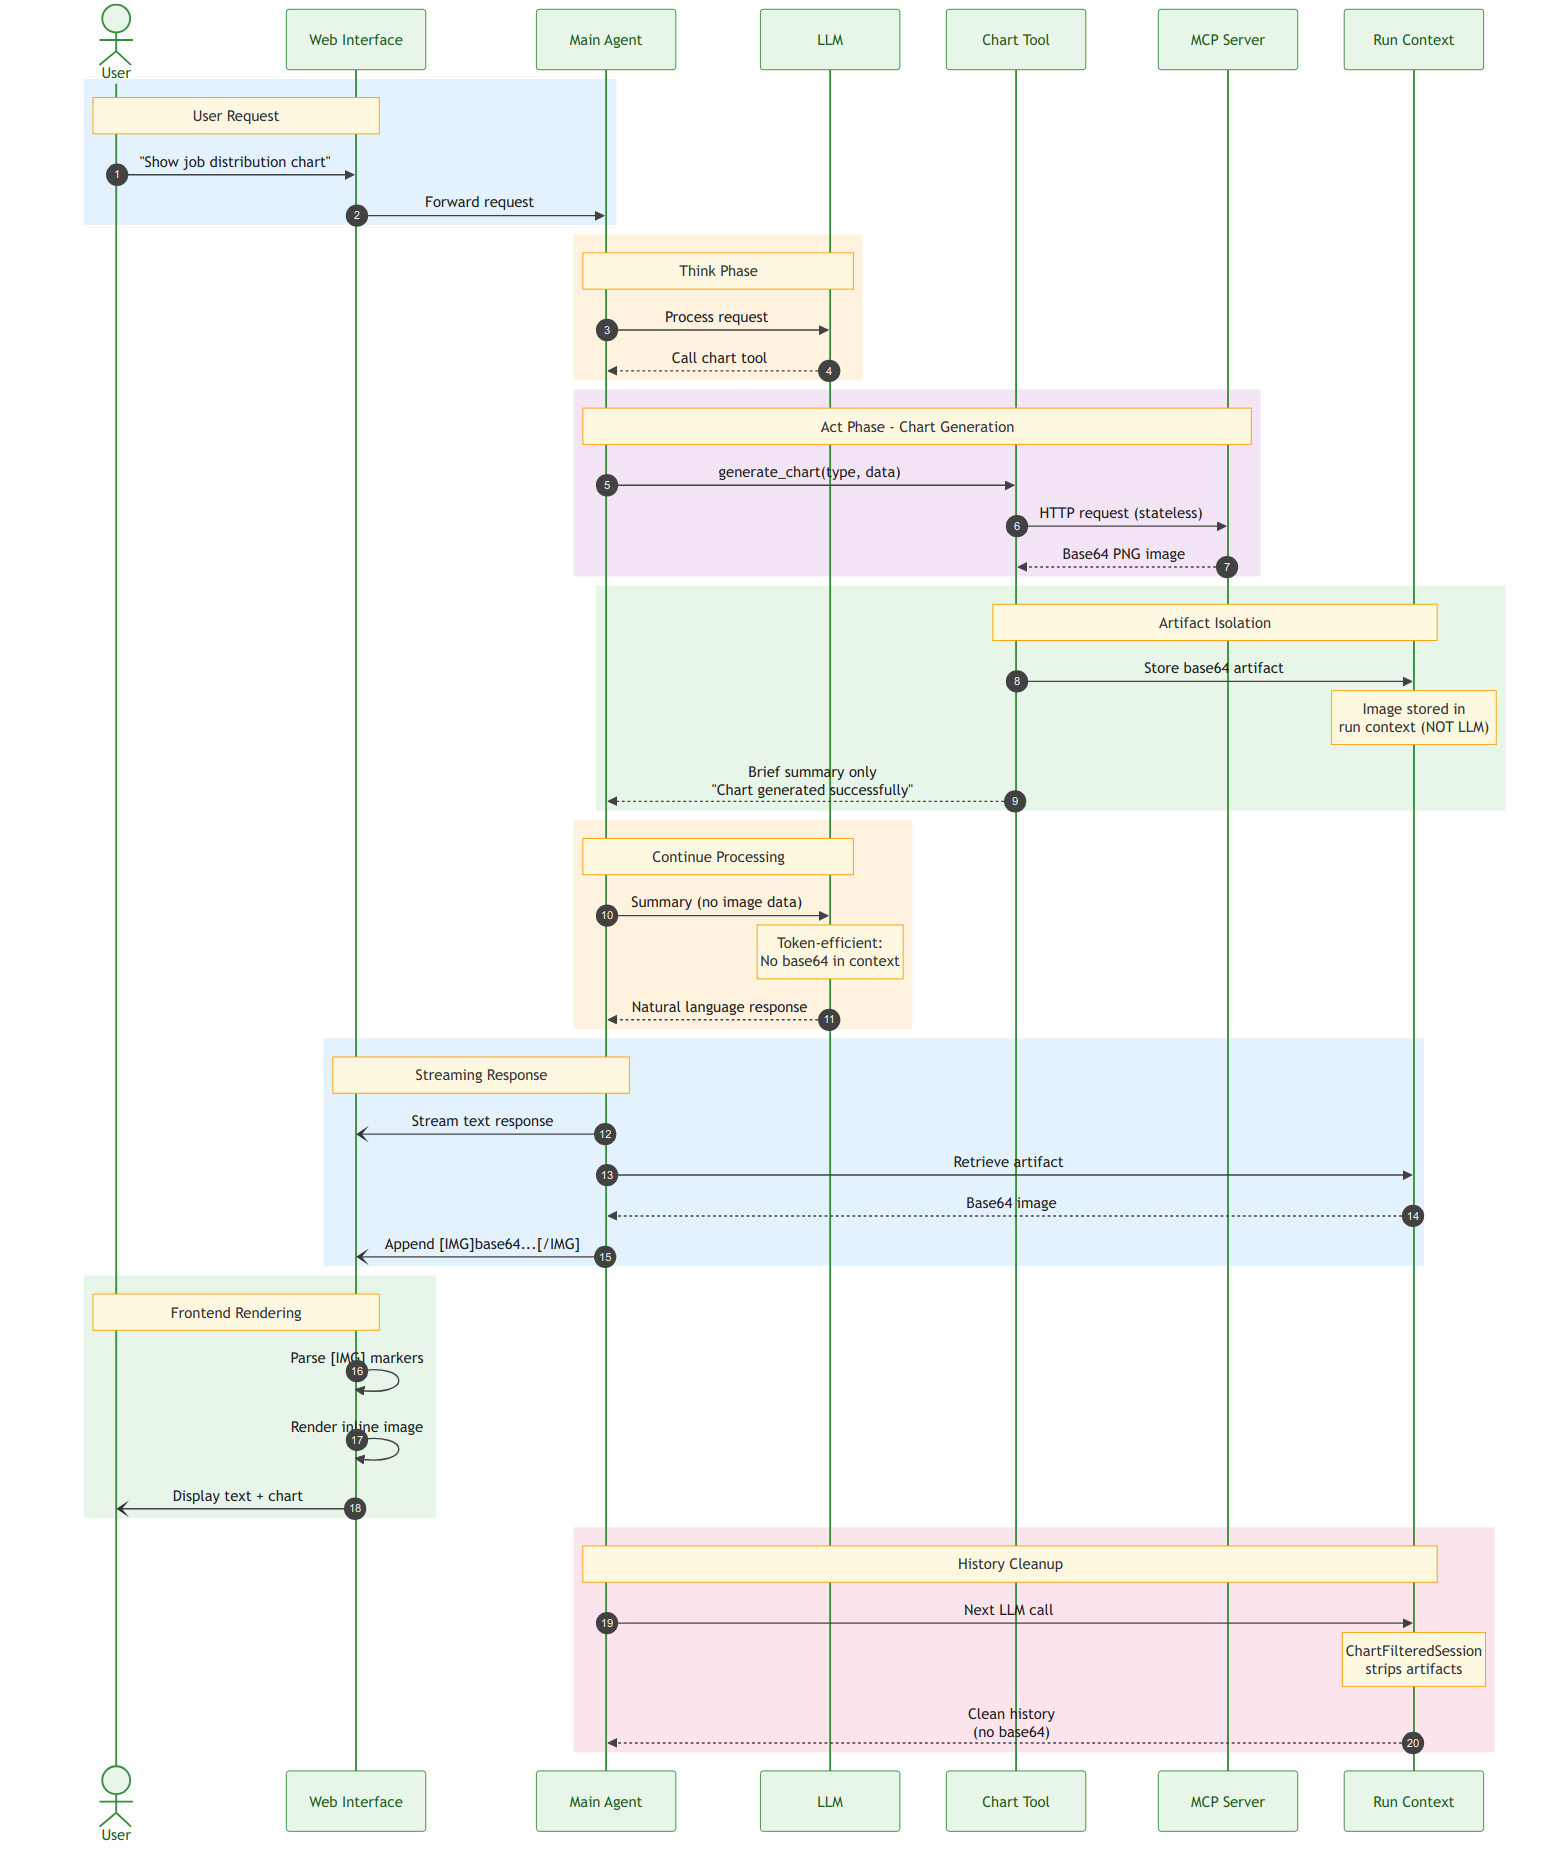
\includegraphics[width=1.3\textwidth]{images/chart_artifact_flow.png}}
    \caption{Chart Artifact Isolation Flow: Separating Visual Data from Conversation Context}
    \label{fig:chart-artifact-flow}
\end{figure}

Chart generation uses direct HTTP calls to the MCP server rather than the SDK flow, as the stateless nature of visualization does not require session context.

\subsection{Session Management and Conversation Persistence}

The backend implements sophisticated session management to support multi-turn conversations with persistent context. Each chat session is identified by a unique session identifier derived from the frontend's chat ID, enabling conversation continuity across page refreshes and reconnections.

Conversation history is stored in SQLite via the OpenAI Agents SDK's \texttt{SQLiteSession} class, wrapped with the \texttt{ChartFilteredSession} to prevent artifact pollution. The session manager implements automatic cleanup of expired sessions (default timeout: one hour) and lazy initialization to avoid unnecessary resource allocation for short-lived interactions.

\subsection{Streaming Response Architecture}

The streaming implementation uses Server-Sent Events to deliver real-time responses to the frontend. This architecture is essential for maintaining responsive user experience during potentially long-running agent operations such as complex cluster analysis or multi-step job management workflows.

The stream format follows OpenAI's chat completion chunk structure for compatibility with existing frontend components. Each chunk includes a unique identifier, timestamp, and delta content. Special event types are encoded within the content field using markers: \texttt{[TOOL:name]} indicates tool invocation, \texttt{[HANDOFF:agent]} indicates agent transition, and \texttt{[IMG]...[/IMG]} encapsulates image artifacts.

Error handling within the streaming context requires particular care, as exceptions must be propagated to the frontend without breaking the SSE connection. The implementation catches exceptions at the generator level, converts them to error event chunks, and gracefully terminates the stream, enabling the frontend to display appropriate error messages while maintaining connection stability for subsequent requests.
